\documentclass{article}
%\usepackage{fullpage}
\usepackage{fancyhdr}
\usepackage[english,francais]{babel}
\usepackage[T1]{fontenc}
\usepackage[utf8]{inputenc}
\usepackage[pdftex]{graphicx}
\usepackage{subfig}

%\renewcommand{\baselinestretch}{2}
\author{Florent \textsc{Guiotte} et Frédéric \textsc{Becker}}
\title{Seam Carving}
\pagestyle{fancy}

\begin{document}
\maketitle
\tableofcontents

\section{Introduction}

Le seam carving est un algorithme de redimensionnement d'image qui permet de garder intact les éléments <<importants>>
de l'image. Cet algorithme utilise une fonction d'énergie (gradient dans notre cas) pour détecter les zones d'intérêts
de l'image.

Dans la première partie de ce TP nous avons travaillé sur l'image verticale 
représentant un loup et la pleine lune (figure \ref{fig:loup}  à la page \pageref{fig:loup}).
Le but de l'algorithme est de rapprocher la lune du loup sans les déformer en réduisant la hauteur de l'image.

\begin{figure}[!ht]%htp]
  \centering
  \subfloat[Image d'origine]{\label{fig:loup}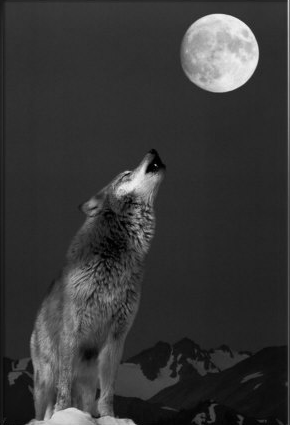
\includegraphics[width=0.48\textwidth]{img/loup.png}}
  \hspace{0.030\textwidth}
  \subfloat[Gradient de l'image]{\label{fig:gradient}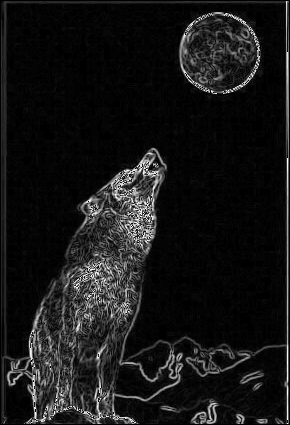
\includegraphics[width=0.48\textwidth]{img/energie.png}}
  \caption{Loup.pgm et calcul de l'énergie associée}
  \label{fig:init}
\end{figure}



\section{Détail de l'algorithme}
\subsection{Fonction d'énergie}
Pour déterminer l'énergie des pixels de l'image nous avons utilisé la mesure du gradient de l'image. Les pixels se
trouvant dans les zones de gradient faible seront éliminés les premiers.

Notre implémentation du calcul de gradient est visible figure \ref{fig:gradient}. On distingue bien les éléments que l'on veut garder de l'image d'origine. L'utilisation du gradient est plutôt efficace dans le cas de cette image.

\subsection{Chemin minimum}
Dans l'algorithme du seam carving, pour réduire la hauteur de l'image d'un pixel, il faut enlever la <<couture>>
horizontale d'énergie minimale.
Pour  déterminer la couture ayant l'énergie la plus faible dans l'image, on utilise l'algorithme de \textsc{Viterbi}.

L'algorithme de \textsc{Viterbi} consiste à sommer les énergies des pixels sur les lignes, en choisissant le pixel ayant
l'énergie la plus faible parmi les trois prédécesseurs (avec une connexité 8) sur la 
colonne précédente. En sélectionnant les plus faibles énergies sommées en fin de ligne, 
on obtiens les coutures horizontales qui représentent le moins d'information dans l'image. 
Ce sont ces coutures qu'ils suffit de supprimer pour obtenir le résultat du seam carving. 
Ces résultats sont visibles figure \ref{seams} sur l'image du loup, sur lequel nous avons 
relancé plusieurs fois le calcul sans supprimer les coutures <<faibles>>.

\begin{figure}[!ht]
    \center
    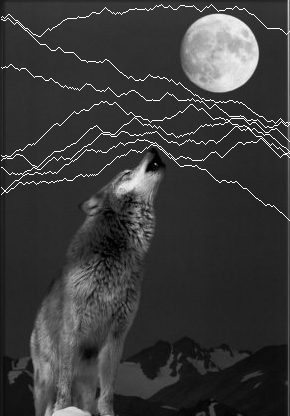
\includegraphics[width=0.48\textwidth]{img/seams.png}
    \caption{Coutures d'énergie minimales}
    \label{seams}
\end{figure}

\subsection{Suppression de la couture}

Une fois la couture minimum relevée, il suffit de la retirer en décalant les colonnes 
d'un pixel vers le haut pour combler la couture manquante, puis de réduire la hauteur totale de l'image.

\begin{figure}[!ht]
    \center
    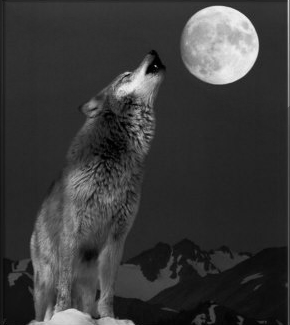
\includegraphics[width=0.48\textwidth]{img/reduced.png}
    \caption{Résultat du seam carving}
    \label{loup_reduced}
\end{figure}

Le résultat sur le loup est visible figure \ref{loup_reduced}, nous avons enlevé 90 lignes 
à l'image d'origine et nous avons bien conservé sans déformation la partie contenant le loup 
et celle contenant la lune.

\section{Améliorations}
\subsection{Masques}

Certains résultats du seam carving ne sont pas satisfaisant, notamment sur une image qui contient
une énergie plus ou moins constante ou si un sujet important pour l'utilisateur est déformé\footnote{Sur la figure \ref{mer:sc} on peut remarquer que le deuxième personnage en partant de la gauche est déformé.}.
Pour garder le contrôle sur les zones à protéger ou à détruire en premier, le moyen le plus 
simple est de définir des masques manuellement.

Sur cette partie, nous avons travaillé sur l'image de la mer (figure \ref{mer:origine}). Pour effectuer des suppressions de coutures verticales nous avons retourné notre image pour conserver notre implémentation. 

\begin{figure}[!ht]%htp]
  \centering
  \subfloat[Image d'origine]{\label{mer:origine}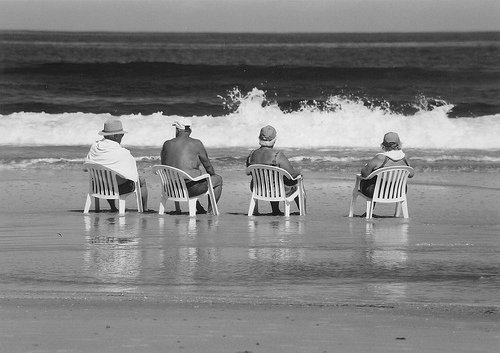
\includegraphics[width=0.48\textwidth]{img/mer.png}}
  \hspace{0.030\textwidth}
  \subfloat[Seam carving basique]{\label{mer:sc}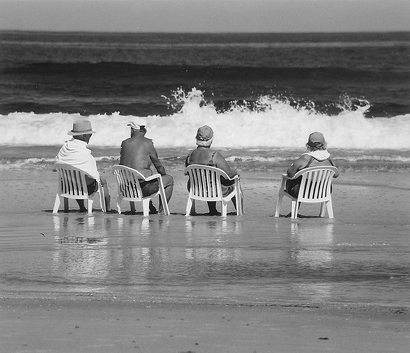
\includegraphics[width=0.48\textwidth]{img/mer_reduced.png}}
  \caption{Mer.pgm et résultat du seam carving}
  \label{mer:init}
\end{figure}

Les masques sont prédéfinis par l'utilisateur (figure \ref{mask:origine}, le masque vert augmente l'énergie tandis que le masque rouge la diminue), on les ouvre en même temps que l'image à
traiter, puis au moment du calcul de l'énergie il suffit d'augmenter ou de diminuer les valeurs
en fonction des valeurs des calques à ces emplacements. Le résultat est visible figure \ref{mask:sc}.


\begin{figure}[!ht]%htp]
  \centering
  \subfloat[Masques]{\label{mask:origine}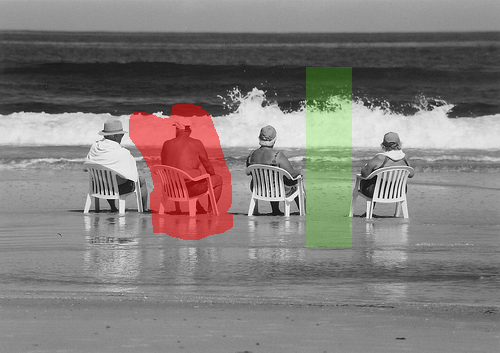
\includegraphics[width=0.7\textwidth]{img/mer_app_mask.png}}
  \hspace{0.030\textwidth}
  \subfloat[Seam carving avec masque]{\label{mask:sc}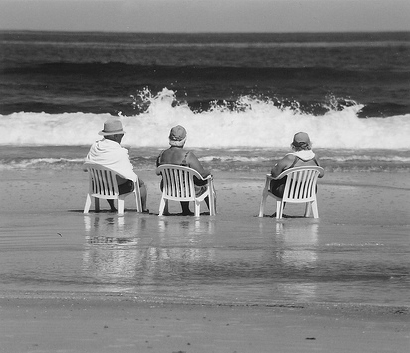
\includegraphics[width=1.0\textwidth]{img/mer_mask_reduced.png}}
  \caption{Application des masques et résultat final}
  \label{mer:init}
\end{figure}

\end{document}
